\documentclass{article}
\usepackage[utf8]{inputenc}
\usepackage[]{hyperref}

\author{
  Raatikka, Marko\\
  \texttt{marko.raatikka@aalto.fi}
  \and
  Lucas, Triefenbach\\
  \texttt{lucas.triefenbach@aalto.fi}
}
\title{Energy efficiency of HTTP2 over HTTP1.1 on the mobile web
\\
\vspace{5mm}
\large{CSE-E5440: Energy-efficient Mobile Computing\\Group C}
}
\date{\today}

\usepackage{natbib}
\usepackage{graphicx}

\begin{document}

\maketitle
\clearpage

\section{Part I}

\subsection{Introduction}
With the increasing computation power and connection speed of mobile phones in recent years, the amount of data flowing through the Internet to mobile end devices continues to grow. While web applications have become ever more complex and the amount of HTML, JavaScript and CSS required to render a web page increases, HTTP1.1 -- the prevailing transfer protocol of today's web -- has failed to keep up with the pace. One of the culprits of HTTP1.1 is that it can only handle one request per a TCP connection and that it can only have a certain maximum number of connections per host (5-8 connections depending on the browser). To work around these shortcomings developers have used techniques such as domain sharding (hosting assets across multiple domains), image spriting and inlining CSS \& JavaScript in the HTML. However, a transport layer problem can not be efficiently solved at the application level.

The work for a new version of HTTP protocol was set forth by Google in 2012 in the form an open networking protocol called SPDY. Later, in 2015, building on the work done for SPDY, HTTP2 was proposed as the future standard protocol. The biggest improvements HTTP2 introduces over HTTP1.1 are request/response multiplexing (to avoid a so called \emph{head-of-line blocking} inherent in HTTP1), header compression, prioritization of requests and server push mechanism. Web services are slowly migrating into adopting HTTP2, but as of today, only about 7\% of the websites have fully migrated to the new protocol. \citep{google-spdy}\citep{http2_stats}\citep{http2}

This work sets to study the impact of HTTP2 on mobile power consumption. Previous work on the topic has been done by \citep{previous_work}. However, this study focuses more on generating high traffic and mimicking common, real-life navigation patterns. Due to time constraints testing is limited to a single browser as opposed to testing across various versions. The content is organized as follows: chapter \ref{chapter:design-implementation} describes the method used, the testbed environment and the test suite. Chapter \ref{chapter:results} continues by presenting the experiment results, which are later reviewed in Chapter \ref{chapter:discussion}. Last, an outline for the part II of the study is given.


\subsection{Design and Implementation}
\label{chapter:design-implementation}

The energy efficiency of the HTTP1.1 and HTTP2 protocols were measured by generating large amounts of network traffic. Six different web services were chosen as the targets, including Flickr, Yahoo, Facebook, Twitter, Weather.com and Instagram. These web services were selected based on their popularity and support for HTTP2 clients (browsers). Facebook, Twitter and Weather.com were eventually omitted from the final experiment corpus: the network traffic generated by Facebook was highly optimized, and therefore, it was assumed that it would not introduce any interesting statistical differences. Twitter on the other hand was deemed too lightweight (consisting of mostly text-based content), while Weather.com suffered from peculiar latency issues when transmitting images over HTTP2 as shown by Figure \ref{fig:weather.com}.

\begin{figure}[h!]
\centering
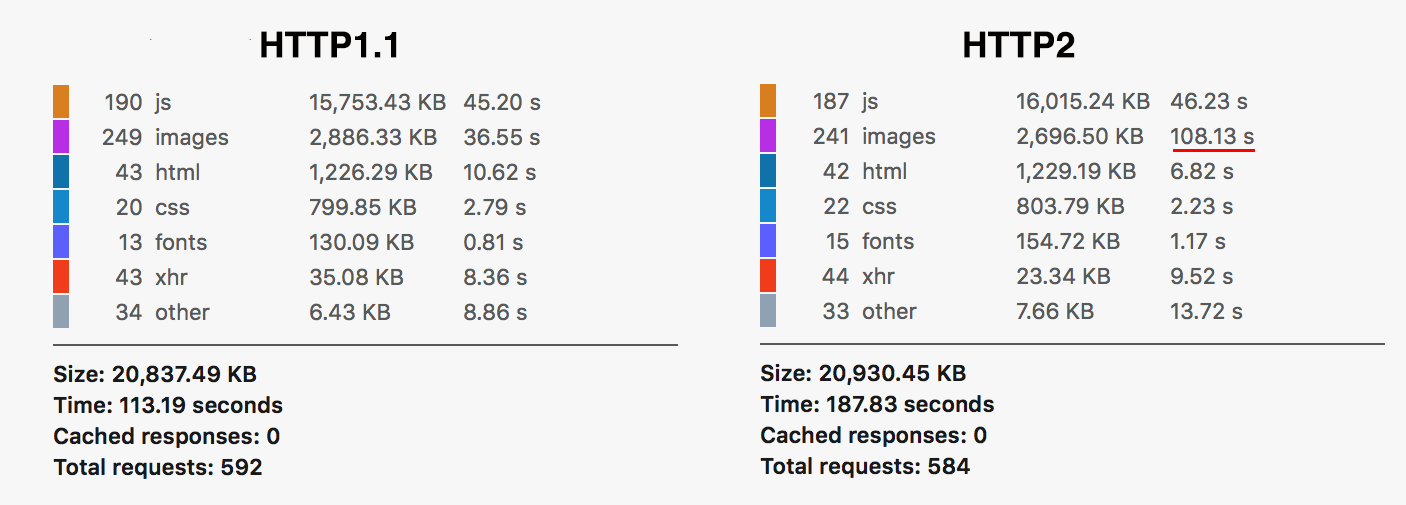
\includegraphics[scale=0.6]{images/weathercom.png}
\caption{Weather.com was excluded from the final experiment corpus because it exhibited abnormally long response times when image assets were fetched over HTTP2. This was done the prevent introducing bias to the energy consumption measurements.}
\label{fig:weather.com}
\end{figure}

The experiment was conducted using Firefox (version 46.0) as, at the time of this writing, no other publicly available browser supports manually disabling HTTP2. The implementation of a robust and reproducible experiment environment required automation of the navigation logic. Browser automation frameworks Appium\footnote{Appium - \url{appium.io}} and Mozilla’s Robocop\footnote{Robocop - \url{https://wiki.mozilla.org/Auto-tools/Projects/Robocop}} were originally considered for this task. However, Appium lacked support for the Firefox browser, and Robocop -- Mozilla’s internal tool for testing Firefox on mobile -- missed proper documentation. Thus, an alternative approach -- including the use of Android’s low level input API -- was taken. The utilization of the input API was inspired by an open-source energy consumption measurement framework called GreenMiner \citep{greenminer}, which uses this technique extensively.

The Android input API allows for the emulation of device gestures, and consequently, automation of browser navigation. The trade-off of this approach is that it requires root access to the device. Therefore the Samsung S4 used for the experiment was rooted using ClockworkMod recovery (version 6.0.4.7) and CyanogenMod (version 12), which ships with Android 5.1.1. The upside of installing a custom ROM -- a customized OS image installed on the device's ROM memory -- like CyanogenMod is that any pre-installed Google services or bundled Samsung software are not included. This helped in minimizing any unwanted power consumption generated by these type of services running in the background unknowingly.

Monsoon Solutions' Power Monitor\footnote{\url{https://www.msoon.com/LabEquipment/PowerMonitor/}} was used for collecting the energy consumption data. The negative and positive terminals of the smartphone battery were connected to the power monitor using copper wire. The two reading terminals of the Samsung S4 battery were isolated with tape to allow the smartphone to be started using external power (the Power Monitor). The experiment scripts used for navigating to the different websites were implemented as Bash shell scripts. The scripts were transferred onto the device via USB using ADB (Android Debug Bridge). ADB also allowed controlling the execution of the test scripts from the laptop, so no human interaction was required while running the tests.

Prior to running the test suite different smartphone features that might have caused noise (e.g. the energy consumption of background processes) were disabled. This included disabling automatic brightness, notifications, sounds, vibrations, widgets, lights and the phone's power saving features. Features enabled for experiment purposes were WiFi, Airplane mode and Developer options. The measurements were conducted in the Aalto open WiFi network during the late evening (22:00) to ensure low latency and minimal network congestion. All caching functionality of the Firefox browser was disabled to maximize network traffic (assets would always be fetched over the network). Crash reporting and monitoring capabilities of the browser were disabled so that they would not cause spikes in power consumption during the experiment. The browser HTTP2 support could be toggled on and off via the Firefox configuration interface. The cache and HTTP configuration flags used are listed in Table \ref{table:firefox_flags}. For further information the interested reader is referred to the MozillaZine Knowledge Base\footnote{MozillaZine Knowledge Base - \url{http://kb.mozillazine.org/}}.

\clearpage

\begin{table}[]
    \centering
    \begin{tabular}{l|c|}
        \textbf{Flag} & \textbf{Value} \\
        browser.cache.check\_doc\_frequency & 1 \\
        browser.cache.disk.enable           & FALSE \\
        browser.cache.memory.enable         & FALSE \\
        network.http.spdy.enabled.http2     & TRUE/FALSE
    \end{tabular}
    \caption{The Firefox configuration flags set in the experiment.}
    \label{table:firefox_flags}
\end{table}

After the smartphone and the laptop have been connected to the Power Monitor and the power measurement UI (Power Tool UI) has been opened the experiment is conducted as follows:

\begin{enumerate}
    \item Start the Power Monitor with an output voltage of 3.7V and sampling rate of 5000Hz
    \item Boot the phone and ensure it has been configured as described above
    \item Connect the smartphone to a laptop via its micro USB connection (for ADB communication)
    \item Install Firefox 46.0 via ADB and configure it as described above (partially automated)
    \item Execute the test suite \emph{n} number of times for either HTTP2 or HTTP1.1 (fully automated).
\end{enumerate}

Upon executing the test suite the power monitoring is manually started via the Power Tool UI for recording the energy consumption of the test run. The rundown of the \emph{test suite} is as follows:

\begin{enumerate}
    \item Close stale instances of Firefox (if any)
    \item Ensure brightness is set to maximum and no screen dim is enabled (a fail-safe mechanism)
    \item Upload experiment scripts to the phone via ADB
    \item Wait $t_{bwt}$ seconds and start Firefox (open at \emph{about:blank})
    \item Wait $t_{nwt}$ seconds and navigate to a target website
    \item Swipe down the page 3-4 times to force dynamic/lazily loaded content to be loaded waiting $t_{swt}$ seconds after each swipe
    \item Navigate to a subpage and wait $t_{nswt}$ seconds
    \item Repeat steps \textbf{6-7} for five different subpages
    \item Navigate to \emph{about:blank} and repeat steps \textbf{5-8} for each target website
    \item Wait $t_{nwt}$ seconds, close Firefox and wait $t_{bwt}$ seconds before concluding the experiment.
\end{enumerate}

The wait times referred to above are given in Table \ref{table:wait_times}. The tap wait time $t_{twt}$ was used when tapping was required for loading more page content (e.g. tapping on a \emph{Load more} button). In addition to running the test suite to gather energy consumption metrics, the test suite was also run separately to capture network traffic (payload sizes, latency, number of requests) via the Firefox WebIDE\footnote{Firefox WebIDE - \url{https://developer.mozilla.org/en-US/docs/Tools/WebIDE}}.

\begin{table}[h!]
    \centering
    \begin{tabular}{l|c|l|}
        \textbf{Variable} & \textbf{Duration (s)} & \textbf{Description} \\
        $t_{nwt}$   & 15    & Navigation wait time \\
        $t_{nswt}$  & 10    & Subpage navigation wait time \\
        $t_{bwt}$   & 5     & Base wait time \\
        $t_{swt}$   & 3     & Swipe wait time \\
        $t_{twt}$   & 2     & Tap wait time
    \end{tabular}
    \caption{Wait time variables used in the experiment.}
    \label{table:wait_times}
\end{table}

\subsection{Results}
\label{chapter:results}

The average network latency -- or Round Trip Time (RTT) -- and packet loss measured when connecting to the three target web services (Yahoo, Instagram, Flickr) via the Aalto open WiFi is presented in Table \ref{table:latency}.

\begin{table}[h!]
    \centering
    \begin{tabular}{c|c|c|c}
         \textbf{Web service} & \textbf{RTT (ms)} & \textbf{RTT std. dev (ms)} & \textbf{Packet loss} \\
        Yahoo   & 158 & 32 & 4.7\% \\
        Instagram  & 116 & 10 & 0.3\% \\
        Flickr & 132 & 12 & 0.3\% \\
    \end{tabular}
    \caption{RTT and packet loss experienced when being connected to the target websites via the Aalto open WiFi during the experiment.}
    \label{table:latency}
\end{table}

For both of the protocols (HTTP1.1 and HTTP2) the test suite was run three times. Figure \ref{fig:smoothed_power} visualizes the average power level for each of the test runs. The average is computed as a moving average using R\footnote{R: statistical computing framework - \url{https://www.r-project.org/}} and a generalized additive model (GAM) provided by the \emph{geom\_smooth()} function of the \emph{ggplot2}\footnote{ggplot2 - \url{http://docs.ggplot2.org/}} plotting library (version 2.1.0). As seen in the figure, it took a total of 400 seconds to complete a single run of the test suite.

Figure \ref{fig:average_power} presents the power levels of a test run done over HTTP1.1. The samples (x-axis) have been averaged so that the average power level is calculated at intervals of 5000Hz (sampling rate of the Power Monitor). That is, each data point represents the average of a segment of 5000 data points (power levels). The smoothed (moving) average is plotted for easier comparison. Observations made on the data are labeled with letters \emph{A-E}. These observations are discussed later in Chapter \ref{chapter:discussion}.

A summary of the mean power and total energy consumption of the three experiment runs for both HTTP2 and HTTP1.1 are given in Table \ref{table:energy_consumption}. The metrics are calculated for samples within the time frame of 24-395 seconds, which corresponds to the time when the first navigation is executed up until the time when navigating off to \emph{about:blank} after the last target website.

For more accurate analysis of the effect of network traffic, Figure \ref{fig:http2_network_traffic} provides a network request pie chart for the payload sizes, latency and number of requests for both HTTP2 and HTTP1.1. This data is based on a single run executed for both HTTP2 and HTTP1.1 in addition to the actual experiment.

\begin{figure}[h!]
\centering
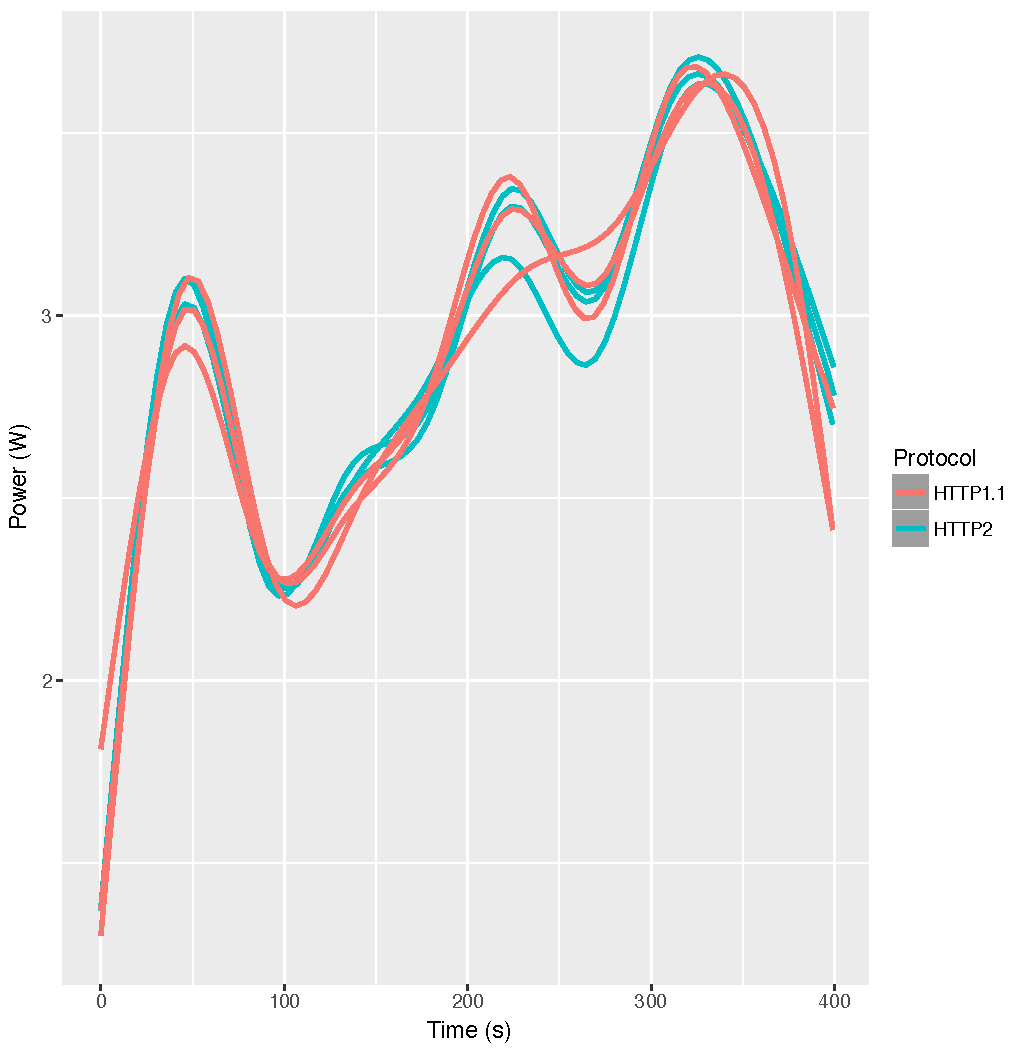
\includegraphics[scale=0.73]{images/smoothed_power}
\caption{Average power level of each six test runs with HTTP2 and HTTP1.}
\label{fig:smoothed_power}
\end{figure}

\begin{figure}[t]
\centering
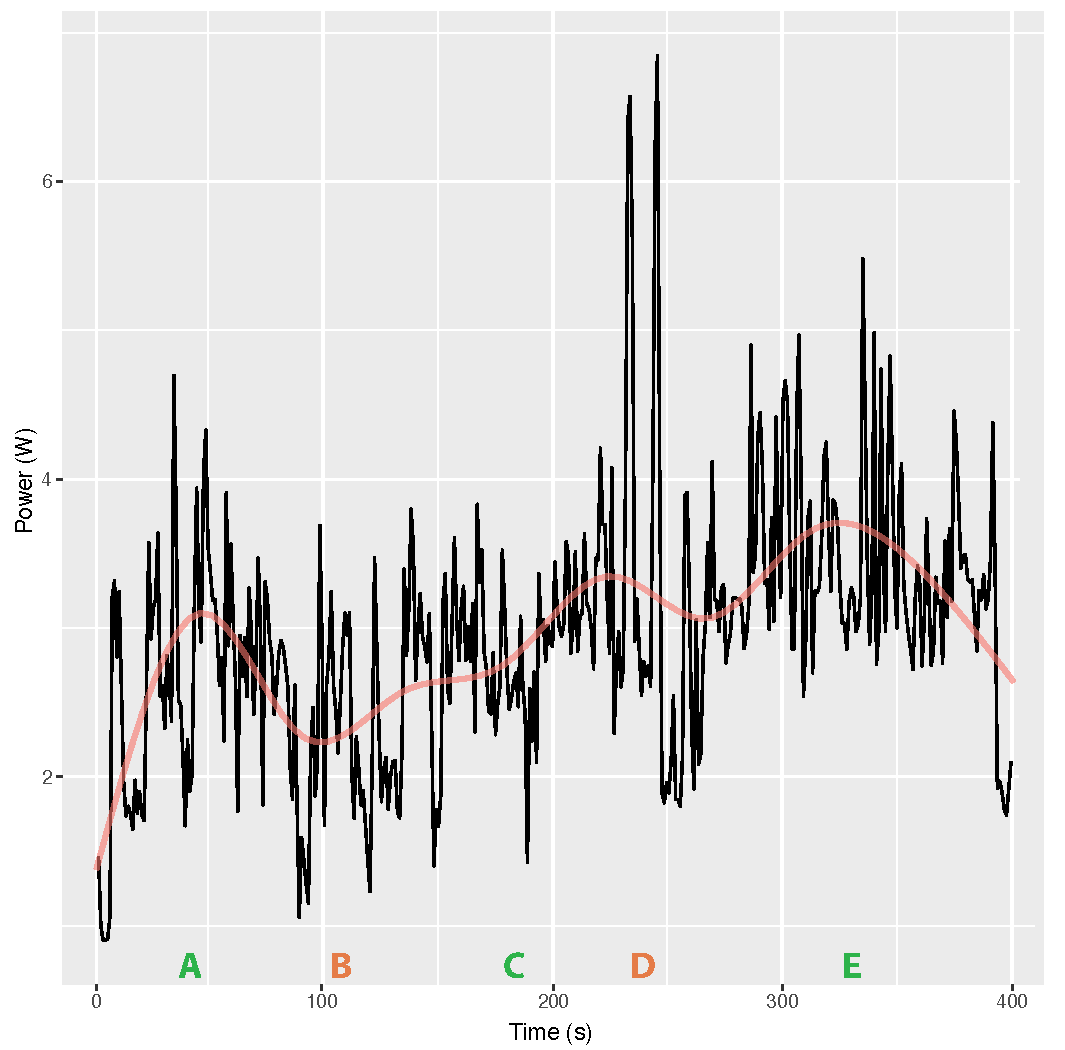
\includegraphics[scale=0.675]{images/average_power}
\caption{Average power levels (of every 1s segment) and the smoothed average of a test run done over HTTP1.1.}
\label{fig:average_power}
\end{figure}

\begin{table}[h!]
    \centering
    \begin{tabular}{c|c|c}
        & \textbf{HTTP1.1} & \textbf{HTTP2}  \\
        Mean (W)   & 2.987 & 2.995 \\
        Std.dev (W) & 0.984 & 1.007 \\
        Total (J)  & 1114.2 & 1117.2 \\
    \end{tabular}
    \caption{Energy consumption of HTTP1.1 and HTTP2 over the time frame of 24-395 seconds (from first navigation up until the exit navigation).}
    \label{table:energy_consumption}
\end{table}

\begin{figure}[h!]
\centering
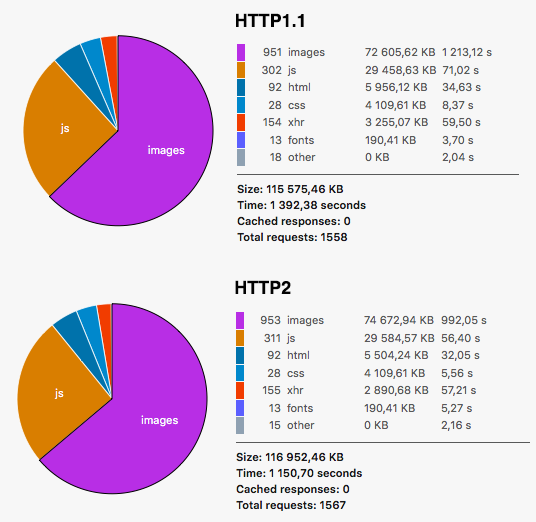
\includegraphics[scale=0.6]{images/http2_consumes.png}
\caption{The network traffic averages for HTTP2 and HTTP1.1 when browsing the target websites.}
\label{fig:http2_network_traffic}
\end{figure}

\clearpage

\subsection{Discussion}
\label{chapter:discussion}

One of the early goals was to compare the energy consumption of the HTTP protocols in different network (latency) conditions as in \cite{previous_work} it was found that significant difference in the energy consumption was observed in the vincinity of 250ms, but not on low or high latencies. The objective was to test if this indeed was the case. Unfortunately however, implementing a setup for reliable latency adjustment (e.g proxying the traffic via VPN) was not done due to time constraints. Therefore, experiments were only performed under the Aalto open WiFi. Another option would have been to force the phone to use a 2G or 3G network. However, 2G proved too unreliable (high packet loss), while 3G actually provided relatively low latency (150ms) similar to that of the Aalto open WiFi connection -- most likely due to the nearby location of the network antenna.

As seen in Table \ref{table:latency} Yahoo exhibited higher latency and significantly higher packet loss. This was believed to be due to the fact that the pages include a relatively high number of ads from various mobile advertisement providers. Furthermore, it can be argued that the CDNs (Content Delivery Network) for Yahoo are less ideally positioned then that of Instagram and Flickr. However, the average latencies are still within a reasonable range (116-158ms) to assume a low latency testbed.

Figure \ref{fig:smoothed_power} shows that the energy consumption difference between the two protocols is minimal. Three runs for both of the protocol is not however enough to draw conclusions. The bump in the average power level for \url{yahoo.com} (also seen in the two power spikes in Figure \ref{fig:average_power}) can be attributed to \emph{layout trashing} observed when swiping down \url{https://yahoo.com/style} on mobile. Unfortunately, this was beyond the control of the authors, so it was later decided that \emph{/style} would be omitted from the subpages to navigate to in any future experiments. One of the HTTP1.1 runs did not seem to spike up in this manner, though, when browsing \url{yahoo.com}. This only goes to tell how important it would be to have had more test runs executed (to minimize the effect of anomalies).

Some interesting observations can be made from the graph in Figure \ref{fig:average_power}. First, it can be seen that the base power of the phone is around 1.20W. Launching and running Firefox increases the base power level to the vincinity of 1.65W (at 12-24 seconds). Labels \emph{A}  and \emph{B} represent the power levels when browsing \url{instagram.com} (at 24-120 seconds). The reason why the power level suddenly drops well below 2W twice (\emph{B}) was due to the fact that the page visited (\url{https://flickr.com/photos/tags}) was light on content, and was actually navigated to twice, consecutively. As the URL would not change when navigated to the second time, Firefox was smart enough to not load the page preserving energy in the process. The fact that this subpage was visited twice in a row was an implementation bug missed by the authors when conducting the tests.

Label \emph{C} and \emph{D} represent the power levels when browsing \url{flickr.com} (at 135-250 seconds). The spikes (\emph{D}) were due to layout trashing as referred to earlier. Last, label \emph{E} represents the browsing of \url{instagram.com} (at 260-395 seconds). Judging by the graph, it seems as if Instagram would be the most energy inefficient. However, as the order of target websites in the corpus was not randomized, such conclusions can not be drawn. It might very well be that the progressive increase in the power level is due to increasing device temperature, or Firefox's excess allocation of memory and/or processes over time.

The energy consumption results summarized in Table \ref{table:energy_consumption} show that the consumption was virtually identical between HTTP2 and HTTP1.1 across the test runs. However, Figure \ref{fig:http2_network_traffic} indicates that HTTP2 was more performant in fetching assets over network. For example, HTTP2 spent 20\% less time on average for fetching assets. It could be argued that the better latency of HTTP2 comes with the price of slightly higher power consumption.

An effort was given to follow the best practices of software energy experimentation as per \textbf{ENERGISE}\footnote{Software energy experimentation best practices: \url{https://github.com/ds4se/chapters/blob/c6f960b5955ef835752f265eed7337ff51cf35e0/abramhindle/energymining.md\#lets-energise-your-software-energy-experiments}} -- a mnemonic coined by the authors of \cite{greenminer}. Due to time constraints the tests were run only on one Firefox version (46.0). Moreover, only three test runs were done for both protocols, which clearly is not enough to draw any statistically significant conclusions. However, in other aspects of the ENERGISE practices the experiment was conducted to the authors' best ability. Especially, the automation of the test suite was a significant achievement, which will help in improving and adjusting the testbed for part II of this study.

In addition to evaluation of potential power saving mechanisms, a few items are left as TODOs for the part II of this study.

\section{Part II}

\emph{Evaluation of potential power saving mechanisms...}
\\ \\
\textbf{TODOs:}
\begin{itemize}
    \item proxy traffic via a VPN to simulate a high latency condition
    \item randomize the order of the target websites in the corpus
    \item increase test run count to at least 10 for better confidence
    \item increase generated network traffic (increase corpus or implement deeper navigation patterns)
    \item evaluation of the effect of HTTP2 best practices on energy consumption
    \item Energy utility (kB/J)
    \item Energy consumption right after high CPU stress (to explain differences in energy consumption per web service)
    \item URL manifest
    \item Average \& std. dev. of network traffic metrics
\end{itemize}
\clearpage

\subsection{Changes to Part I}
\begin{itemize}
    \item added a subpage navigation to instagram.com
    \item removed swiping prior to navigation
    \item collected granular network data for a URL manifest
\end{itemize}

\subsection{Runtimes}
\begin{itemize}
    \item Yahoo: 150 s
    \item Flickr: 170 s
    \item Instagram: 200 s
\end{itemize}


\subsection{Results}

% Latencies (avg. & std.dev)

    % Aalto open (w/o VPN)
    % instagram.com     112.747         4.708
    % yahoo.com         133.282         8.004
    % flickr.com        131.587         6.611

    % Aalto closed (w/ VPN)
    % instagram.com     295.559         56.325
    % yahoo.com         303.997         77.832
    % flickr.com        306.019         50.457

\begin{table}[h!]

    \begin{tabular}{lll}
        \textbf{Site} & \textbf{Visit duration (s)} & \textbf{Payload (kB)} \\
        \hline \vspace{-3mm}\\
        \textbf{https://flickr.com} \\
        \hspace{1em} /expore \\
        \hspace{1em} /photos/tags/primavera \\
        \hspace{1em} /photos/tags/amazing \\
        \hspace{1em} /photos/tags/rural \\
        \hspace{1em} /photos/tags/brazil \vspace{1mm}\\
        \textbf{https://instagram.com} \\
        \hspace{1em} /nhl \\
        \hspace{1em} /binghuiliu \\
        \hspace{1em} /jordanspieth \\
        \hspace{1em} /warriors \\
        \hspace{1em} /nba \\
        \hspace{1em} /ufc \vspace{1mm}\\
        \textbf{https://yahoo.com} \\
        \hspace{1em} /nhl \\
        \hspace{1em} /tech \\
        \hspace{1em} /news \\
        \hspace{1em} /business \\
        \hspace{1em} /tv \vspace{1mm}\\
    \end{tabular}
    \caption{Energy consumption of HTTP1.1 and HTTP2 over the time frame of 24-395 seconds (from first navigation up until the exit navigation).}
    \label{table:url_manifest}
\end{table}
TBD

\subsection{Proposal for Improvements}
TBD

\subsection{Conclusions}
Turning on the Performance governor to ensure a more static high CPU level lead to instability, and could not therefore be used.
TBD

\bibliographystyle{plain}
\bibliography{references}
\end{document}
